\subsection{Transforming Coordinate Systems}
\label{key:data:cs}
Usually, \PGFPlots\ works with cartesian coordinates. However, one may want to provide coordinates in a different coordinate system.

In this case, the |data cs| key can be used to identify the input coordinate system:

\begin{pgfplotskey}{data cs=\mchoice{cart,polar,polarrad} (initially cart)}
	Defines the coordinate system (`cs') of the input coordinates. \PGFPlots\ will apply transformations if \meta{name} does not match the expected coordinate system.
\begin{codeexample}[]
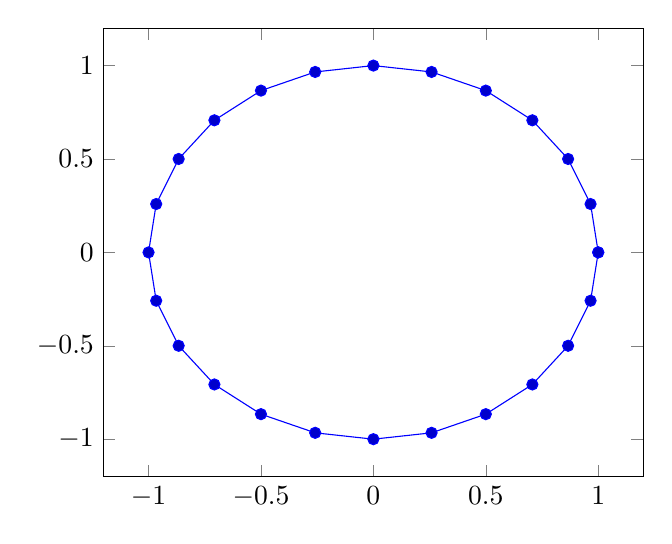
\begin{tikzpicture}
	\begin{axis}
	\addplot+[data cs=polar,domain=0:360] (\x,1);
	\end{axis}
\end{tikzpicture}
\end{codeexample}
\begin{codeexample}[]
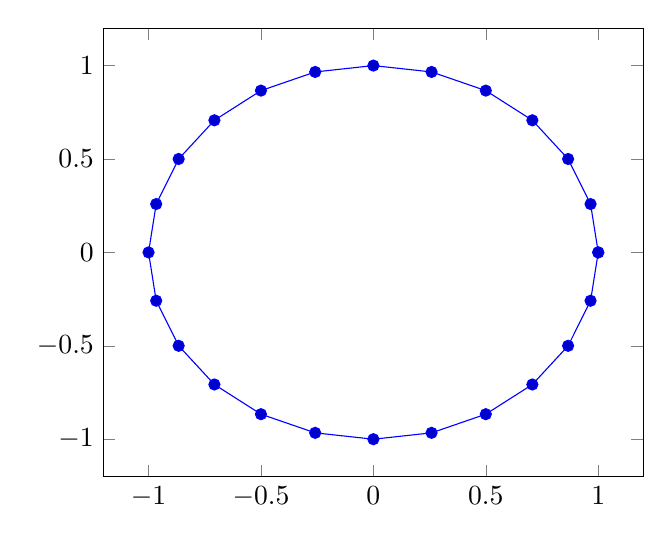
\begin{tikzpicture}
	\begin{axis}
	\addplot+[data cs=polarrad,domain=0:2*pi] (\x,1);
	\end{axis}
\end{tikzpicture}
\end{codeexample}
	Every axis type has its own coordinate system. For example, a normal |axis| expects the |cart| coordinate system, whereas a |polaraxis| expects a |polar| coordinate system. If the argument to |data cs| does not match the expected coordinate system, \PGFPlots\ will transform it:
% \usepgfplotslibrary{polar}
\begin{codeexample}[]
% requires \usepgfplotslibrary{polar}
\begin{tikzpicture}
	\begin{polaraxis}
	\addplot coordinates {(90,1) (180,1)};
	\addplot+[data cs=cart] 
		coordinates {(1,0) (0.5,0.5)};
	\end{polaraxis}
\end{tikzpicture}
\end{codeexample}
	
	At the time of this writing, \PGFPlots\ supports the following values for \meta{name}:

	The |data cs=|\declareandlabel{cart} denotes the cartesian coordinate system. It is expected by the usual |axis| (or its logarithmic variants). It can have three components, $x$, $y$, and $z$.

	The |data cs=|\declareandlabel{polar} is the (two--dimensional) coordinate system with (angle, radius). The angle is a periodic number in the range $[0,360)$; the radius is any number. If a |polar| coordinate has a $z$ component, it is taken as-is (the transformations ignore it).

	The |data cs|=\declareandlabel{polarrad} is similar to |polar|, but it expects the angle in radians, i.e.\ in the periodic range $[0,2\pi)$.

	At the point of this writing, the |data cs| method will work for most plot handlers. But for complicated plot handlers, further logic may be needed which is not yet available (for example, the |quiver| plot handler might not be able to convert its direction vectors correctly)\footnote{In case you run into problems, consider writing a bug report or ask others in \TeX\ online discussion forums.}.
\end{pgfplotskey}

\begin{command}{\pgfplotsaxistransformcs\marg{fromname}\marg{toname}}
	Expects the current point in a set of keys, provided in the coordinate system \meta{fromname} and replaces them by the same coordinates represented in \meta{toname}.

	On input, the coordinates are stored in |/data point/x|, |/data point/y|, and |/data point/z| (the latter may be empty). The macro will test if there is a declared coordinate transformation from \meta{fromname} to \meta{toname} and invoke it. If there is none, it will attempt to convert to |cart| first and then from |cart| to \meta{toname}. If that does not exist either, the operation fails.
\end{command}

\begin{command}{\pgfplotsdefinecstransform\marg{fromname}\marg{toname}\marg{code}}
	Defines a new coordinate system transformation. The \meta{code} is expected to get input and write output as described for |\pgfplotsaxistransformcs|.

	Implementing a new coordinate system immediately raises the question in which math mode the operations shall be applied. \PGFPlots\ supports different so--called ``coordinate math systems'' for generic operations, and for each individual coordinate as well. These coordinate math systems can either use basic \PGF\ math arithmetics, the |fpu|, or perhaps there will come a Lua\TeX\ library.

	The documentation of this system is beyond the scope of this manual\footnote{Which is quite comprehensive even without API documentation, as you will certainly agree...}. Please consider reading the source-code comments and the source of existing transformations if you intend to write own transformations.
\end{command}
